\documentclass[tikz,border=8pt]{standalone}
% Shared look for every TikZ diagram. Load with \input{../../tools/tikz-style.tex}
\usepackage[sfdefault]{roboto}
\usetikzlibrary{arrows.meta, positioning, shapes.geometric, calc, fit, backgrounds}
\definecolor{cblue}{HTML}{4C78A8}
\definecolor{corange}{HTML}{F58518}
\definecolor{cgreen}{HTML}{54A24B}
\definecolor{cred}{HTML}{E45756}
\definecolor{cpurple}{HTML}{B279A2}
\definecolor{cgrey}{HTML}{6B6B6B}
\tikzset{
  every picture/.style={font=\sffamily, line width=1.2pt},
  box/.style={draw=#1, fill=#1!12, rounded corners=4pt, align=center, inner sep=7pt, minimum height=1.1cm},
  box/.default=cgrey,
  arrow/.style={-{Stealth[length=3mm]}, draw=cgrey, line width=1.4pt},
  title/.style={font=\sffamily\bfseries\Large},
  note/.style={font=\sffamily\small, text=cgrey, align=center},
}
\AtBeginDocument{\hyphenpenalty=10000 \exhyphenpenalty=10000}

% The forces on the pushed cup (side view, drawn 50 times its size): the push F to the left at height p, the
% weight mg down through the centre, the table's upward support N and the friction f to the right along the base.
% O is the left bottom corner, the corner the cup would tip over. Left: push at p = 0.04 m, the push's torque about O
% is 0.0392 N m, less than the weight's 0.0736 N m, so the cup slides. Right: push at p = 0.08 m, 0.0785 N m, more
% than 0.0736 N m, so the cup tips.
\begin{document}
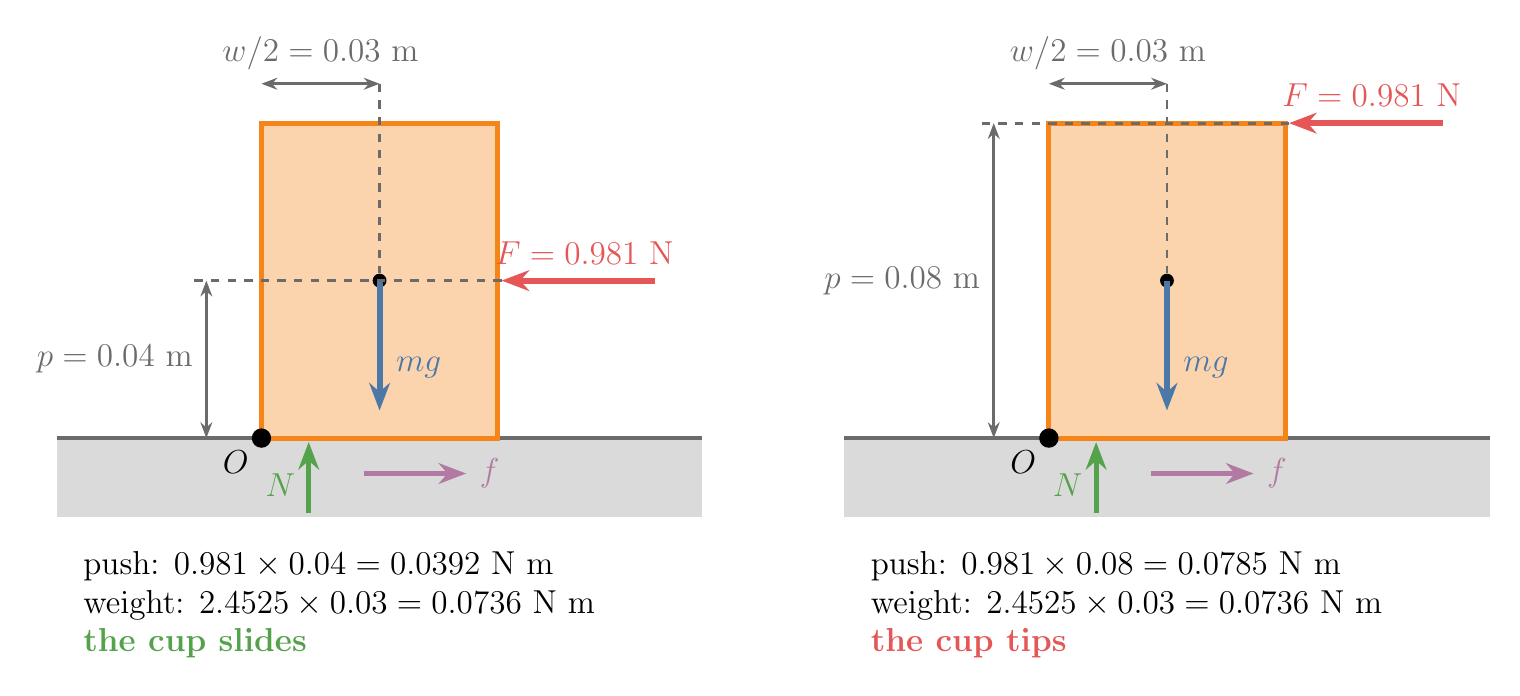
\begin{tikzpicture}[every node/.append style={font=\large}]
  \foreach \xs/\p/\pl/\tq/\verdict/\vcol in {0/2/0.04/0.0392/slides/cgreen, 10/4/0.08/0.0785/tips/cred} {
    \begin{scope}[xshift=\xs cm]
      % table and cup
      \fill[cgrey!25] (-2.6,-1.0) rectangle (5.6,0);
      \draw[cgrey, line width=1.5pt] (-2.6,0) -- (5.6,0);
      \draw[corange, fill=corange!35, line width=1.8pt] (0,0) rectangle (3,4);
      % pivot O
      \fill[black] (0,0) circle (3.5pt);
      \node[below left=1pt] at (0,0) {$O$};
      % weight through the centre
      \fill[black] (1.5,2) circle (2.5pt);
      \draw[-{Stealth[length=3.5mm]}, line width=2.2pt, cblue] (1.5,2) -- (1.5,0.35);
      \node[cblue, right=2pt] at (1.5,0.9) {$mg$};
      % push at height p, pointing left, applied at the right face
      \draw[-{Stealth[length=3.5mm]}, line width=2.2pt, cred] (5.0,\p) -- (3.05,\p);
      \node[cred, above=2pt] at (4.1,\p) {$F = 0.981$ N};
      % support and friction at the base (drawn under the cup)
      \draw[-{Stealth[length=3.5mm]}, line width=1.8pt, cgreen] (0.6,-0.95) -- (0.6,-0.05);
      \node[cgreen, left=1pt] at (0.6,-0.6) {$N$};
      \draw[-{Stealth[length=3.5mm]}, line width=1.8pt, cpurple] (1.3,-0.45) -- (2.6,-0.45);
      \node[cpurple, right=1pt] at (2.6,-0.45) {$f$};
      % lever arms
      \draw[cgrey, line width=1pt, dashed] (3.05,\p) -- (-0.9,\p);
      \draw[cgrey, line width=1.2pt, {Stealth[length=2mm]}-{Stealth[length=2mm]}] (-0.7,0) -- (-0.7,\p);
      \node[cgrey, left=1pt] at (-0.7,\p/2) {$p = \pl$ m};
      \draw[cgrey, line width=1.2pt, {Stealth[length=2mm]}-{Stealth[length=2mm]}] (0,4.5) -- (1.5,4.5);
      \node[cgrey, above=1pt] at (0.75,4.5) {$w/2 = 0.03$ m};
      \draw[cgrey, line width=1pt, dashed] (1.5,4.5) -- (1.5,2.1);
      % torques about O
      \node[align=left, anchor=north west] at (-2.4,-1.3) {push: $0.981 \times \pl = \tq$ N m\\
        weight: $2.4525 \times 0.03 = 0.0736$ N m\\ \textcolor{\vcol}{\textbf{the cup \verdict}}};
    \end{scope}
  }
\end{tikzpicture}
\end{document}
